\section{\large\textbf{Results}}
\subsection{Sample}
The sample consisted of 33 participants. From the demographic data collected, shown in Figure \ref{fig:demografico}, responses were obtained from 22 participants who reported working or studying in a sound-related field. Only 2 participants completed the test under noisy conditions. Regarding the headphones used during the test, 20 participants used On-ear/Over-ear headphones, while the rest used In-ear headphones. For the devices used during the test, 10 participants used a mobile phone, 10 used a computer, and 13 used a computer with an external audio interface. The majority of participants reported listening to music with headphones, while only 6 stated they did not engage in this activity. In the case of surround sound systems, the opposite trend was observed; only 14 participants reported using surround sound systems, with 11 of them doing so less than once per week.

\begin{figure}[H]
    \centering
    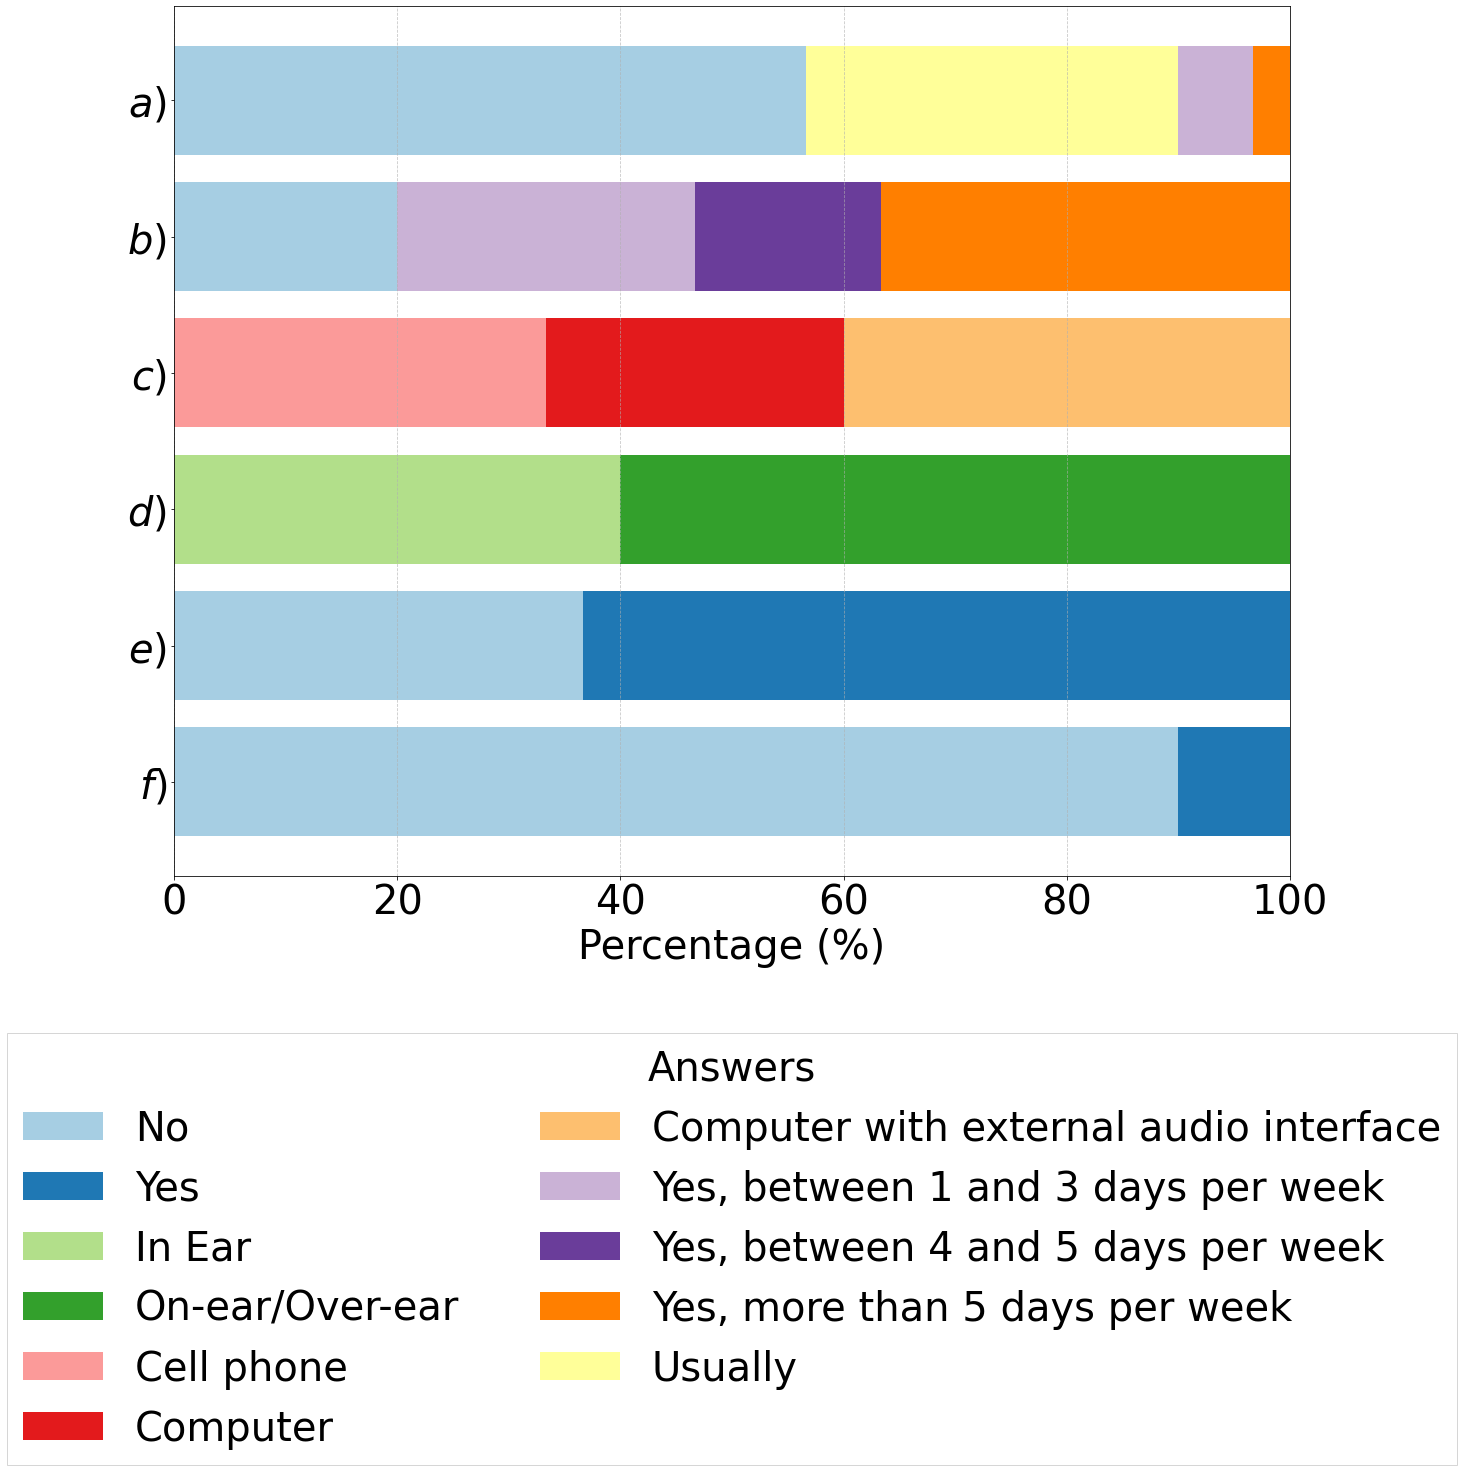
\includegraphics[width=0.65\textwidth]{Figures/prueba.png}
    \caption{Demographic distribution obtained for each question.}
    \label{fig:demografico}
\end{figure}

\subsection{Data Analysis}
Regarding the localization test conducted, the overall accuracy rate distribution is shown in Figure \ref{fig:porcentajeQ}. It was verified that this distribution does not follow a normal distribution, as determined by a Shapiro-Wilk test (p-value $<$ 0.05). Additionally, the distribution of correct responses for each source directivity was evaluated using the same method and criterion, resulting in a non-normal distribution for each directivity. For this reason, results from participants whose scores for more than one source directivity were identified as outliers (according to the interquartile range criterion) were excluded. Based on this criterion, a total of 3 participants were removed.


\begin{figure}[H]
    \centering
    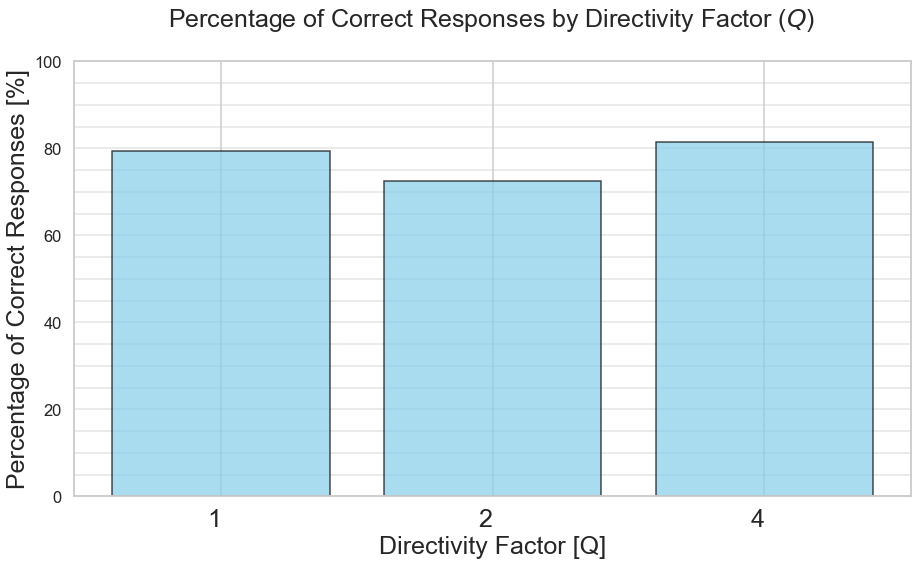
\includegraphics[width=0.65\textwidth]{Figures/PorcentajeQ.png}
    \caption{Percentage of correct answers for each directivity factor.}
    \label{fig:porcentajeQ}
\end{figure}

The decrease in the percentage of correct responses between directivity 1 and directivity 2 is 8\%, while the increase between directivity 2 and 4 is 11\%. A $\chi^2$ analysis was performed to determine whether the directivity factor significantly influenced localization ability, resulting in a p-value $<$ 0.05, confirming it as a significant factor.

The correct responses by frequency were also analyzed, as shown in Figure \ref{fig:porcentajeF}. This figure reveals a considerable decrease in accuracy rates within the 250 Hz band, while bands at 400 and 500 Hz show an improvement in localization ability for the source with directivity 4.

\begin{figure}[H]
    \centering
    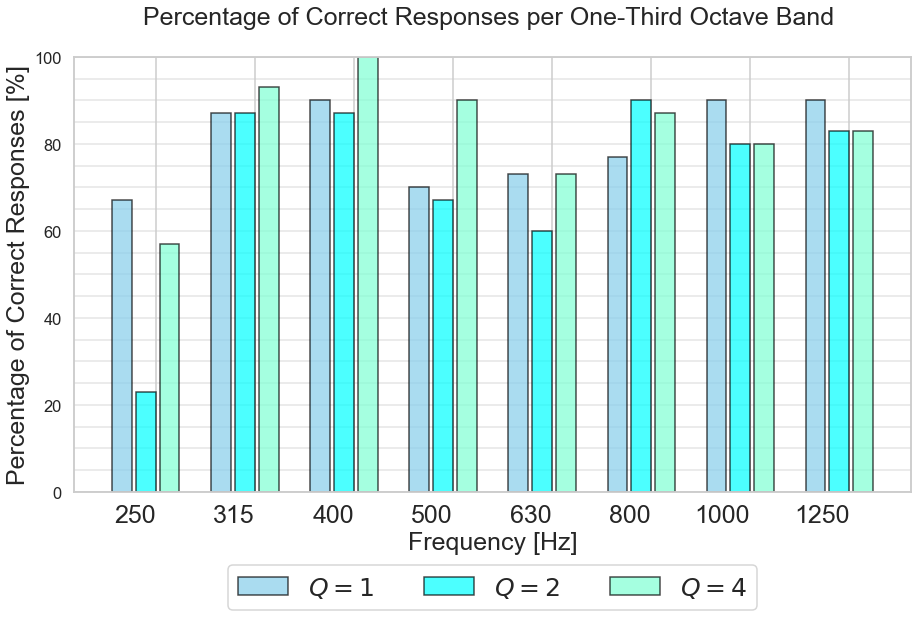
\includegraphics[width=0.65\textwidth]{Figures/tercios.png}
    \caption{Percentage of correct answers for each third-octave.}
    \label{fig:porcentajeF}
\end{figure}

Separate $\chi^2$ analyses were conducted for each demographic question. Significant differences (p-value $<$ 0.05) were found for the type of headphones used, with an overall accuracy increase of 7.8\%. Figure \ref{fig:porcentaje_aur} shows the frequency differences obtained for each type of headphone.

Additionally, significant differences were observed in the device used during the test, specifically between mobile phones and computers/computers with an external audio interface, with an 11\% increase for computers. No differences were found between the computer and the computer with external audio interface groups. Figure \ref{fig:porcentaje_disp} shows the percentage of correct answers for each device used.

\begin{figure}[H]
    \centering
    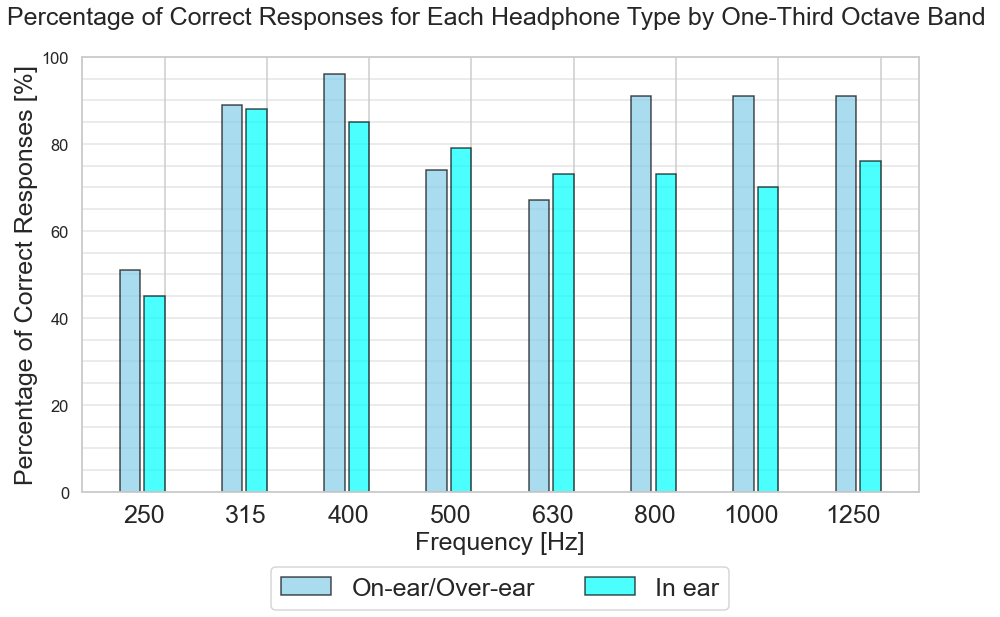
\includegraphics[width=0.65\textwidth]{Figures/auriculares.png}
    \caption{Percentages of correct answers for each type of headphone used.}
    \label{fig:porcentaje_aur}
\end{figure}

For participants who study or work in a sound-related field, a significant 10\% difference in accuracy was noted compared to those who do not, with the latter achieving 71.7\% accuracy and the former reaching 81.9\%.

\begin{figure}[H]
    \centering
    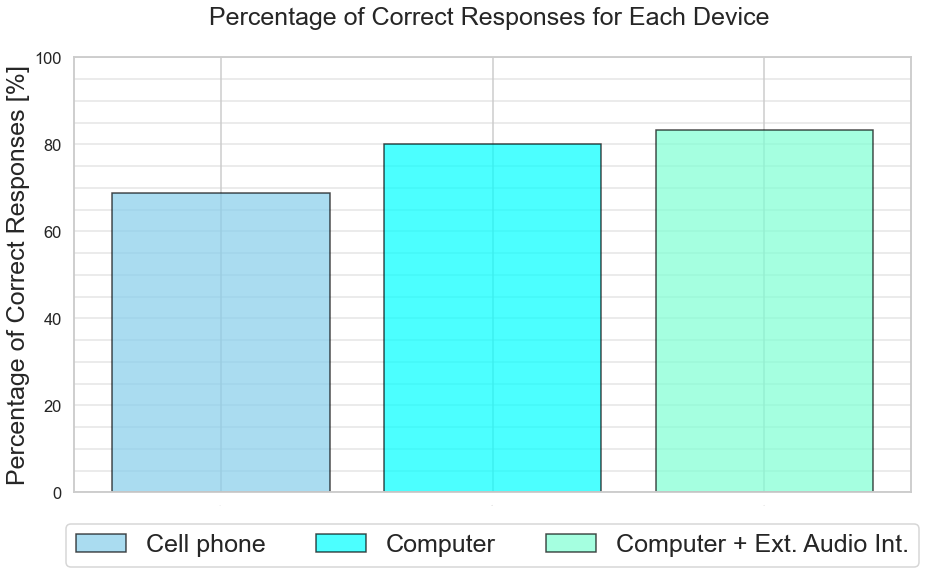
\includegraphics[width=0.65\textwidth]{Figures/dispositivos.png}
    \caption{Percentages of correct answers for each device used.}
    \label{fig:porcentaje_disp}
\end{figure}

Lastly, for participants who reported listening to surround sound systems multiple times a week, a significant difference was noted, favoring those who answered "no" with an average difference of 15\%. Figure \ref{fig:porcentaje_surround} shows the percentage of correct answers by frequency of surround sound listening. No differences were found for the other demographic questions.

\begin{figure}[H]
    \centering
    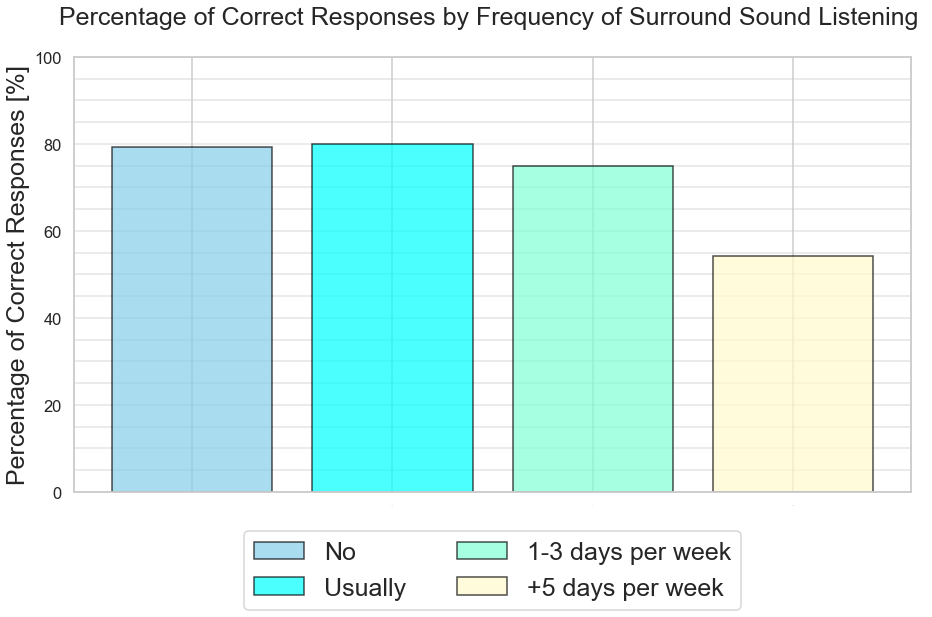
\includegraphics[width=0.65\textwidth]{Figures/surround.png}
    \caption{Percentages of correct answers by frequency of surround sound listening.}
    \label{fig:porcentaje_surround}
\end{figure}
